\secrel{Светодиоды}

\noindent
\begin{tabular}{p{0.7\textwidth}p{0.3\textwidth}}
\noindent\parbox[b]{0.65\textwidth}{В настоящее время светоизлучающие диоды
используются в индикаторах и дисплеях на различном оборудовании, однако они все
больше и больше используются в качестве замены для \termdef{галогенных
ламп}{лампа!галогенная} и \termdef{ламп
накаливания}{лампа!накаливания}\note{использующие светящиеся проводники внутри
стеклянных колб} во многих других приложениях. Они включают в себя ходовые огни
на транспорте, светофоры,  большие уличные TV-экраны.}&
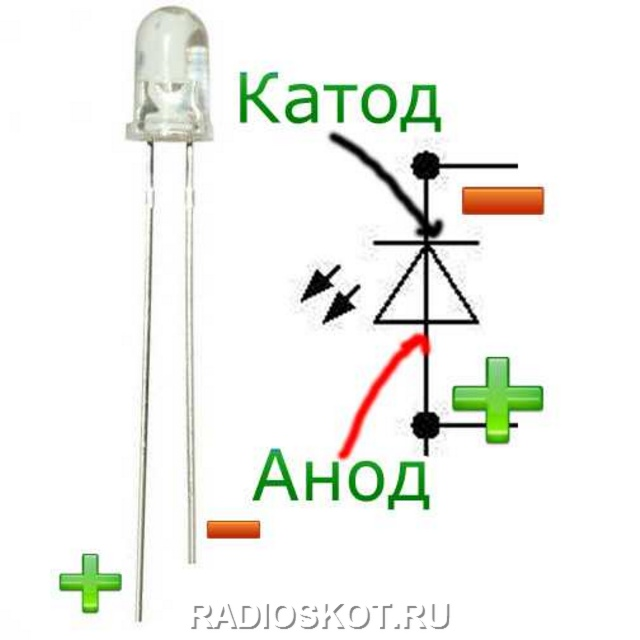
\includegraphics[width=0.25\textwidth]{bcollis/led.jpeg}
\\
\end{tabular}

\noindent
\begin{tabular}{p{0.3\textwidth} p{0.7\textwidth}}
\noindent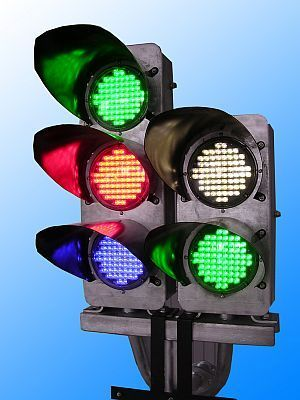
\includegraphics[width=0.3\textwidth]{bcollis/ledtraffic.jpeg}&
\noindent\parbox[b]{0.65\textwidth}{По сравнению с \term{лампами накаливания},
светодиоды почти не дают тепла, и поэтому очень эффективны. Они также имеют
гораздо б\'{о}льшее время жизни, например 10 лет, по сравнению с 10 месяцами для
ламп накаливания. Таким образом, в некоторых ситуациях например сигналов
светофора, если там установлены светодиоды, они дают значительную экономию как
по потребляемой мощности, так и по стоимости технического обслуживания. Хотя
есть небольшая проблема со светодиодными светофорами\ --- они не плавят снег,
который на них налипает!}\\
\end{tabular}
